\documentclass[12pt,a4paper]{article}
\usepackage[utf8]{inputenc}
\usepackage{amsmath}
\usepackage{amsfonts}
\usepackage{amssymb}
\usepackage{enumerate}
\usepackage[T1]{fontenc}
\usepackage{graphicx}
\usepackage{polski}
\usepackage{url}
\usepackage{array}
\usepackage{hyperref}
\usepackage{float}



\addtolength{\hoffset}{-1.5cm}
\addtolength{\marginparwidth}{-1.5cm}
\addtolength{\textwidth}{3cm}
\addtolength{\voffset}{-1cm}
\addtolength{\textheight}{2.5cm}
\setlength{\topmargin}{0cm}
\setlength{\headheight}{0cm}
\title{Dokumentacja projektu ZPI}
\begin{document}

\title{Dokumentacja projektu ZPI}
\author{Bartłomiej Tokarczyk |
Mateusz Sromek |
Wojciech Sułowski |
Maciej Więcławek}
\date{\today}

\maketitle
\begin{abstract}
Dokumentacja projektowa z przedmiotu zespołowe przedsięwzięcie inżynierskie realizowanego w Państwowej Wyższej Szkole Zawodowej Nowy Sącz. Założeniem projektu jest utworzenie aplikacji mobilnej o nazwie Singiel 2.0. Aplikacja służy do zawierania nowych znajomości z innymi użytkownikami oraz  komunikowania między sobą poprzez wiadomości tekstowe i rozmowy wideo. Prowadzącym przedmiot jest mgr inż. Nikodem Bulanda.
\end{abstract}
\newpage

\tableofcontents
\listoftables
\listoffigures

\newpage

\section{Tytuł}
SINGIEL 2.0
\section{Nazwa robocza}
Aplikacja randkowa z komunikatorem
\section{Cel}
Stworzenie aplikacji do łączenia w pary użytkowników z możliwością czatowania
\\
\\
SINGIEL 2.0 to aplikacja pełna możliwości. Możemy zawierać znajomości poprzez parowanie się użytkowników. Jeśli chcesz poszerzyć krąg towarzyski, spotkać się z kimś i poznawać nowych ludzi to znajdujesz się we właściwym miejscu. Funkcja przesuń w prawo aby kogoś polubić,a jeśli ktoś odwzajemni Twoje polubienie - jesteście parą. Ktoś nie za bardzo Ci się spodobał? Funkcja przesuń w lewo aby kogoś odrzucić.
\section{Zakres}
\subsection{Analiza wymagań}
\hspace{10mm}Aplikacja mobilna umożliwiająca łączenie/parowanie się z innymi użytkownikami 
aplikacja umożliwia czatowanie, prowadzenie rozmów wideo (Web RTC - kamerka)
możliwość przesyłania kontaktów przy pomocy technologii NFC
szyfrowanie wiadomości czatu (klient-serwer)
przesyłanie plików i multimediów (zdjęcia, filmy)



\hspace{10mm}Użytkownik na samym początku ma możliwość rejestracji konta singla. Po wpisaniu odpowiednich wymagań (imię, wiek, dodanie zdjęcia, zainteresowań, ustalenia hasła) staje się zalogowanym, pełnoprawnym właścicielem konta singla.
Aplikacja ma umożliwiać przeglądanie profili użytkowników poprzez główną stronę widoczną dla użytkownika po zalogowaniu.Tutaj wyświetlane będą propozycje do sparowania się z drugą osobą poprzez wyświetlanie ich zdjęcie wraz z imieniem, wiekiem i opisem. Singiel ma możliwość odrzucenia danej osoby lub jej akceptacji. By porozmawiać z osobą której daliśmy szansę poznania, musi odwzajemnić parowanie. W przypadku odrzucenia jednej z osób nie ma możliwości czatowania z druga osobą. 
Poza stroną główną, zalogowany klient ma możliwość przeglądania zakładek “czat” oraz “edycja profilu”. Zakładka czat wyświetla wszystkich użytkowników połączonych w pary. Poprzez wybranie osoby do czatowania mamy możliwość konwersacji tekstowej z drugą osobą, rozmowy wideo, przesyłania plików oraz przesyłania kontaktów technologią NFC. Ponadto, użytkownik aplikacji posiada możliwość zablokowania kontaktu z osobą uprzednio połączoną w pary. Edycja profilu to zakładka, w której istnieje możliwość zaktualizowania zdjęcia, profilu oraz aktualizowania opisu użytkownika. Po wypełnieniu formularza oraz akceptacji nowo wprowadzonych informacji, następuje proces aktualizacji profilu który jest wyświetlany innym użytkownikom aplikacji. W zakładce “edycja profilu” użytkownik może zrezygnować z posiadania konta w aplikacji poprzez wybranie odpowiedniego przycisku oraz potwierdzeniu swojej decyzji. Aplikacja umożliwia również zmianę hasła, jest to wykonywane przez wypełnienie formularza zawierającego takie pola jak stare hasło oraz dwukrotnie nowe hasło. Formularz sprawdza czy hasła wprowadzone w polach nowe hasło są takie same oraz czy stare hasło zgadza się z tym wprowadzonym podczas rejestracji/uprzedniej zmianie hasła. Dzięki wykorzystaniu technologii Web RTC\cite{webrtcWikipedia} mamy możliwość komunikacji w czasie rzeczywistym z drugą osobą. Platforma Firebase\cite{firebase} zostanie wykorzystana do zintegrowania z naszą usługą. System ten wykorzystuje synchronizację danych co milisekundę co zapewnia absolutną szybkość i wysoką wydajność.
Do implementacji skorzystamy z zintegrowanego środowiska programistycznego Android Studio. Do stworzenia layoutu aplikacji wykorzystamy XML\cite{xml}


\subsection{Deasemblacja}

\begin{itemize}\itemsep0pt
\item [\textbf{*}] Rejestracja i tworzenie profilu \textbf{MVP}
\\ 
\newline
Po zainstalowaniu aplikacji na urządzeniu mobilnym użytkownik otrzymuje możliwość utworzenia konta w aplikacji poprzez kliknięcie przycisku „Zarejestruj się”.  Po rozpoczęciu procesu rejestracji zostaje kolejno przeprowadzony  przez odpowiednie panele zawierające formularze, które zbiorą niezbędne dane na temat użytkownika i przekażą je prosto do bazy danych, która realizowana oraz zarządzana będzie z poziomu platformy oferującej usługi bazodanowe  Firebase.  
\\ 
\item [\textbf{*}] Logowanie \textbf{MVP}
\\ 
\newline
Zarejestrowany użytkownik, po uruchomieniu aplikacji otrzymuje możliwość zalogowania się po kliknięciu przycisku „Zaloguj się”. Po wprowadzeniu poprawnych danych logowania do formularza (adresu e-mail oraz hasła), formularz zostaje przesłany dzięki odpowiednim funkcjom i zapytaniom do bazy danych, dane zostaną obsłużone przez kolejne funkcje i zapytania,  jeśli użytkownik istnieje w bazie oraz wprowadził poprawne dane – zostaje przekierowany do aplikacji. Jeśli wprowadzone dane nie są poprawne, aplikacja poinformuje o tym oraz poprosi o ponowne wprowadzenie danych.
\newline
\item [\textbf{*}] Edycja profilu \textbf{MVP}
\\ 
\newline
Po zalogowaniu się do swojego konta, użytkownik ma możliwość po wejściu w panel edycji profilu, edytować swój profil – edytować wszystkie dane zamieszczone na swój temat w swoim profilu.
\newline 
\item [\textbf{*}] Zmiana zdjęcia \textbf{MVP}
\\ 
\newline
Dzięki odpowiednim, zaimplementowanym funkcjom, użytkownik po zalogowaniu ma możliwość edycji zdjęcia – po kliknięciu odpowiedniego przycisku użytkownik ma możliwość wybrania zdjęcia z galerii swojego urządzenia mobilnego i zamiany z obecnym zdjęciem profilowym.
\newline
\item [\textbf{*}] Zmiana opisu \textbf{MVP}
\\ 
\newline
Po zalogowaniu użytkownik ma możliwość zmiany opisu, w panelu edycji profilu, w odpowiednim miejscu, posiada możliwość edycji tekstu i podmienienia go z obecnym.
\newline
\item [\textbf{*}] Przeglądanie użytkowników (swipe up) \textbf{MVP}
\\ 
\newline
Główna funkcja aplikacji, po zalogowaniu użytkownik posiada możliwość akceptacji/odrzucenia drugie użytkownika. Akceptacja oznacza chęć nawiązania kontaktu i dodanie do „sparowanych” między sobą osób – możliwość kontaktu tekstowego oraz rozmów wideo. Odrzucenie skutkuje brakiem tych funkcjonalności między odpowiednimi użytkownikami.
\newline
\item [\textbf{*}] Czat \textbf{MVP}
\\ 
\newline
Po zalogowaniu oraz pozytywnym sparowaniu się z innym użytkownikiem, użytkownik otrzymuje możliwość wymiany wiadomości tekstowej na czacie, wszystkie wiadomości są szyfrowane.  Czat obsługiwany będzie przez  platformę Firebase.
\newline

\item [\textbf{*}] Usuwanie konta \textbf{MVP}
\\ 
\newline
Po zalogowaniu się, użytkownik ma możliwość usunięcia konta w aplikacji, po kliknięciu odpowiedniego przycisku i uwierzytelnieniu za pomocą hasła, za pomocą odpowiednich funkcji i zapytań wysłanych do bazy danych – konto i wszystkie dane na jego temat zostają usunięte z bazy danych.
\newline
\item [\textbf{*}] Zmiana hasła \textbf{MVP}
\\ 
\newline
Po zalogowaniu się, oraz przejściu do panelu zmiany hasła, użytkownik po autoryzacji przez podanie starego hasła oraz dwukrotnie (dla potwierdzenia) nowego hasła ma możliwość jego zmiany. Cała operacja zmiany hasła obsługiwana jest przez odpowiednie funkcje oraz zapytania wykonujące operacje na bazie danych.
\newline
\item [\textbf{*}] Blokowanie użytkowników
\\ 
\newline
Użytkownik posiada możliwość zablokowania użytkownika, z którym wcześniej się sparował. Po zablokowaniu innego użytkownika nie ma możliwości jakiegokolwiek kontaktu między zablokowanymi.
\\ 
\newline
\item [\textbf{*}] Przesyłanie kontaktów za pomocą NFC
\\ 
\newline
Przy wykorzystaniu technologii NFC, po zbliżeniu telefonów na odpowiednią odległość, użytkownicy posiadają możliwość przesłania sobie danych kontaktowych.
\newline
\newpage
\item [\textbf{*}] Rozmowa Live
\\ 
\newline
Przy wykorzystaniu technologii WebRTC po sparowaniu się, użytkownicy mają możliwość przeprowadzenia między sobą rozmowy wideo – przesył obrazu oraz dźwięku między użytkownikami.
\newline

\item [\textbf{*}] Przesyłanie multimediów
\\ 
\newline
Użytkownik, po zalogowaniu się oraz będący sparowany z innym użytkownikiem, posiada możliwość za pomocą czatu przesłać pliki multimedialne, które posiada na swoim urządzeniu mobilnym.
\newline
\item [\textbf{*}] Layout aplikacji
\\ 
\newline
Layout aplikacji zrealizowany przy pomocy technologii XML, wcześniej zainicjalizowany poglądowo w wersji roboczej dzięki platformie Figma.
\newline

\item [\textbf{*}] Testy aplikacji
\\ 
\newline
Aplikacja w fazie końcowej posiada pozytywnie zaliczone testy manualne.

\end{itemize}
\subsection{Wymagania}

\subsubsection{Funkcjonalne }

\begin{itemize}\itemsep0pt
\item [--]aplikacja umożliwia użytkownikowi rejestrację oraz logowanie
\item [--]aplikacja umożliwia edycję profilu 
\item [--]aplikacja umożliwia zmianę hasła oraz usunięcie konta 
\item [--]aplikacja umożliwia użytkownikom parowanie się z innymi użytkownikami aplikacji 
\item [--]aplikacja umożliwia czatowanie oraz prowadzenie rozmów wideo 
\item [--]aplikacja umożliwia przesyłanie kontaktów za pomocą technologii NFC
\item [--]aplikacja szyfruje wiadomości czatu
\item [--]aplikacja umożliwia przesyłanie plików oraz multimediów
\end{itemize}

\subsubsection{Niefunkcjonalne}

\begin{itemize}\itemsep0pt
\item [--] Dostęp do internetu
\item [--] Urządzenie mobilne z systemem Android  (wersja 6.6 wzwyż)

\item [--] Ukończone 18 lat przez użytkownika
\end{itemize}

\newpage
\subsection{Diagram przypadków użycia i diagram przepływu}

\begin{figure}[h]
\centering
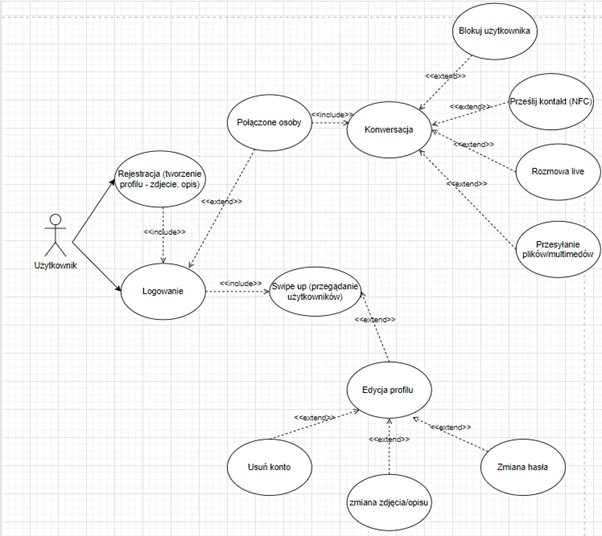
\includegraphics[width=14cm]{zdjęcia i skriny/uml2.jpg}
\caption{Diagram UML}
\end{figure}
\begin{figure}[h]
\centering
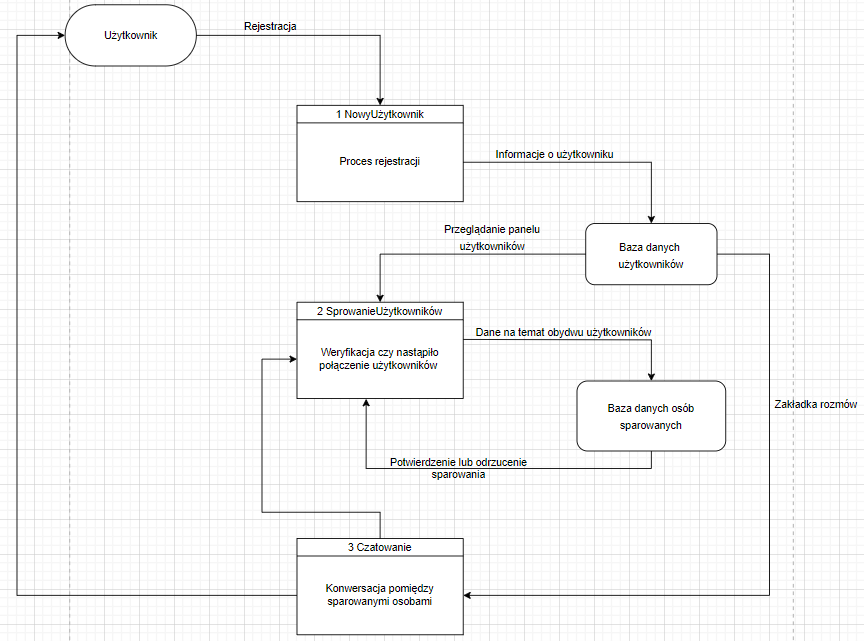
\includegraphics[width=16cm]{zdjęcia i skriny/DataFlowDiagram.png}
\caption{Diagram przepływu}
\end{figure}
\newpage
\subsection{Dobór technologii}

\subsection*{\center\textbf{JAVA}}
\hspace{10mm}Język programowania umożliwiający tworzenie aplikacji na platformę android\cite{java1}, jego głównymi cechami są współbieżność, zastosowanie klas, obiektowość. Java jest oficjalnym językiem programowania aplikacji mobilnych - android oraz jest wspierana przez środowisko pracy Android Studio. W przypadku aplikacji mobilnych język Java jest kompilowany poprzez wirtualną maszynę Dalvik, który od wersji 5.0 Lollipop został zastąpiony poprzez Android Runtime (ART)\cite{java2}.

\subsection*{\center\textbf{Firebase (bazy danych)}}
\hspace{10mm}Firebase jest to platforma umożliwiająca tworzenie aplikacji mobilnych oraz internetowych.  \cite{firebase}
Platforma oferuje użytkownikom kilka przydatnych funkcjonalności, główne z nich to:\\
\\
\textbf{Uwierzytelnianie} - dzięki tej funkcji jesteśmy w stanie określić sposób autoryzacji użytkowników chcących zalogować się do naszej aplikacji \\
\textbf{Baza danych} - bazodanowa funkcja, która umożliwia przechowywanie danych, które wprowadzane są przez użytkowników za pośrednictwem formularzy oraz przycisków \\
\textbf{Składowanie} - moduł ten umożliwia nam przechowywanie plików \\
\textbf{Hosting} - dzięki tej funkcjonalności mamy możliwość wdrożenia prostej strony internetowej a także złożonej aplikacji internetowej    \\
\textbf{Funkcje} - ten moduł pozwala na kompilację kodu po stronie Firebase’a bez konieczności posiadania serwera zewnętrznego  

\subsection*{\center\textbf{WebRTC}}
\hspace{10mm} WebRTC to komunikacja internetowa w czasie rzeczywistym\cite{webrtc}, jest to darmowy projekt typu open source, który jest używany w większości nowoczesnych przeglądarek, pozwalająca użytkownikom komunikować się w czasie rzeczywistym ze sobą bezpośrednio z przeglądarki, aplikacji bez użycia serwera. Za pomocą prostego interfejsu programowania API, którego celem jest zaprojektowanie protokołu, który łączy się typu peer-to-peer, bez konieczności instalacji wtyczek jak i innych aplikacji.\\
\\ 
\textbf{Wykorzystywane oprogramowanie:}
\begin{itemize} \itemsep-5pt
\item Android Studio
\item GitHub
\item Latex (\url{https://www.overleaf.com})
\item Scenariusz UML (\url{https://app.diagrams.net})
\item Layout aplikacji (\url{https://www.figma.com})
\item Jira (\url{https://singiel2k21.atlassian.net})
\end{itemize}

\newpage
\section{Scenariusze}

\begin{table} [H]
\centering
\begin{tabular}{|r|p{9cm}|} \hline
Nr scenariusza & 1 \\
\hline
Tytuł & Utworzenie konta\\
\hline
Aktor/Grupa & Użytkownik \\
\hline
Warunki wejściowe & Użytkownik ma więcej niż 18 lat. \\
\hline
Przebieg/Opis & 
\begin{enumerate}[a)]
\item Po uruchomieniu aplikacji użytkownik wybiera opcję “Zarejestruj się”
\item Użytkownik wpisuje adres email.
\item Użytkownik wprowadza hasło, które spełnia wymogi.
\item Wypełnia formularz dotyczący imienia, daty urodzenia, płci.
\item Użytkownik wybiera płeć osób, które mają mu się wyświetlać.
\item Aplikacja prosi o wpisanie miasta.
\item Użytkownik wybiera swoje zainteresowania (hobby).
\item Wybranie zdjęć jakie mają się wyświetlać po wejściu w profil użytkownika.


\end{enumerate}
\\
\hline
Zakończenie - poprawne & Użytkownik posiada konto w aplikacji.
\\ 
\hline
Zakończenie alternatywne nr: 1 & Użytkownik wpisał hasło niespełniające wymogów -> alert “hasło nie spełnia wymagań”
\\
\hline
Zakończenie alternatywne nr: 2 & Użytkownik wpisał datę urodzenia z której wynika, że ma mniej niż 18 lat -> alert o wymaganym wieku, zamknięcie formularza rejestracji.
\\
\hline
Zakończenie alternatywne nr: 3 & Użytkownik nie wpisał miasta -> alert o braku danych
\\
\hline
Zakończenie alternatywne nr: 4 & Użytkownik nie wybrał zdjęcia profilu -> alert o konieczności wybrania zdjęcia
\\
\hline
\end{tabular}
\caption{Scenariusz "Tworzenie konta".}
\label{table:1}
\end{table}

\begin{table} [H]
\centering
\begin{tabular}{|r|p{9cm}|} \hline
Nr scenariusza & 2 \\
\hline
Tytuł & Swipe up - przeglądanie użytkowników \\
\hline
Aktor/Grupa & Użytkownik \\
\hline
Warunki wejściowe & Użytkownik ma utworzone konto w aplikacji Singiel 2.0  \\
\hline
Przebieg/Opis & 
\begin{enumerate}[a)]
\item Po uruchomieniu aplikacji użytkownik loguje się na swój profil (autologowanie)
\item Użytkownik przechodzi do “swipowania”
\item Aplikacja wyświetla innych użytkowników wraz ze zdjęciem, imieniem, wiekiem i opisem profilu.
\item Użytkownik wybiera spośród wyświetlonych profili. Jeśli chce poznać daną osobę - przesuwa w prawo (akceptuje). Jeśli osoba mu się nie spodobała i nie spełnia oczekiwań - przesuwa w lewo (odrzuca)
\item System po zaakceptowaniu (bądź odrzuceniu) wyświetla kolejne profile użytkowników 


\end{enumerate}
\\
\hline
Zakończenie - poprawne & Użytkownik wykonuje swipe
\\ 
\hline
Zakończenie alternatywne nr: 1 & Niepoprawne wykonanie gestu - użytkownik nie przesunął w żadną stronę przez co nowy profil się nie wyświetlił.
\\
\hline
Zakończenie alternatywne nr: 2 & Użytkownik stracił połączenie internetowe. Nowe profile się nie odświeżają. 
\\

\hline
\end{tabular}
\caption{Scenariusz "Swipe up - przeglądanie użytkowników".}
\label{table:2}
\end{table}





\begin{table} [H]
\centering
\begin{tabular}{|r|p{9cm}|} \hline
Nr scenariusza & 3 \\
\hline
Tytuł & Edycja profilu  \\
\hline
Aktor/Grupa & Użytkownik \\
\hline
Warunki wejściowe & Użytkownik jest zalogowany na swoim koncie. \\
\hline
Przebieg/Opis & 
\begin{enumerate}[a)]
\item Po uruchomieniu aplikacji użytkownik wybiera opcję “Edytuj profil”
\item Aplikacja umożliwia poprzez przycisk edycje wybranych zasobów profilu
\item Użytkownik edytuje profil 
\begin{enumerate}
    \item Użytkownik zmienia zdjęcie
    \item Użytkownik edytuje dane personalne  
    \item Użytkownik edytuje opis 
  \end{enumerate}
\item Użytkownik zatwierdza zmiany 
\end{enumerate}
\\
\hline
Zakończenie - poprawne & Aplikacja wykonuje update, informacje o profilu zostały zaktualizowane.  
\\ 
\hline
Zakończenie alternatywne nr: 1 & Użytkownik po wprowadzeniu zmian nie zatwierdził ich przez anulowanie operacji edycji  -> strona początkowa zakładki “Edycja profilu”.
\\
\hline
Zakończenie alternatywne nr: 2 & Użytkownik nie podał wszystkich obowiązkowych danych -> aplikacja domaga się uzupełnienia danych
\\
\hline
Zakończenie alternatywne nr: 3 & Użytkownik anulował edycję danych  -> powrót do strony głównej zakładki “Edycja profilu”. 
\\
\hline
\end{tabular}
\caption{Scenariusz "Edycja profilu".}
\label{table:3}
\end{table}




\begin{table} [H]
\centering
\begin{tabular}{|r|p{9cm}|} \hline
Nr scenariusza & 4 \\
\hline
Tytuł & Czatowanie \\
\hline
Aktor/Grupa & Użytkownik \\
\hline
Warunki wejściowe & Dopasowanie się użytkowników \\
\hline
Przebieg/Opis & 
\begin{enumerate}[a)]
\item Użytkownik przechodzi do czatu
\item W czat zostają wyświetlenii osoby sparowane z użytkownikiem
\item Użytkownik wybiera  osobę do czatowania
\item Użytkownik wprowadza tekst w wyznaczonym polu
\item Użytkownik wysyła zawartość wiadomości
\end{enumerate}
\\
\hline
Zakończenie - poprawne & Wiadomość została wysłana poprawnie
\\ 
\hline
Zakończenie alternatywne nr: 1 & Użytkownik nie posiada sparowanych osób-> powrót do strony głównej
\\
\hline
Zakończenie alternatywne nr: 2 & Użytkownik wysyła wiadomość do osoby która nie jest już z nim sparowana -> wyświetlenie komunikatu z informacją o braku sparowania z danym odbiorcą
\\
\hline
\end{tabular}
\caption{Scenariusz "Czatowanie".}
\label{table:4}
\end{table}



\begin{table} [H]
\centering
\begin{tabular}{|r|p{9cm}|} \hline
Nr scenariusza & 5 \\
\hline
Tytuł & Rozmowa live \\
\hline
Aktor/Grupa & Użytkownik \\
\hline
Warunki wejściowe & Dopasowanie się użytkowników, Użytkownik posiada kamerę i mikrofon
 \\
\hline
Przebieg/Opis & 
\begin{enumerate}[a)]
\item Po uruchomieniu aplikacji użytkownik wybiera opcję “Chat
\item W czat zostają wyświetlenii osoby sparowane z użytkownikiem
\item Użytkownik wybiera  osobę do czatowania
\item Użytkownik wybiera opcję rozmowy online
\item Aplikacja prosi o zezwolenie na użycie kamery oraz mikrofonu
\item Użytkownik będący odbiorcą połączenia akceptuje połączenie
\item Użytkownik kończy rozmowę klikając w przycisk ‘słuchawki’
\end{enumerate}
\\
\hline
Zakończenie - poprawne & Rozmowa live odbyła się
\\ 
\hline
Zakończenie alternatywne nr: 1 & Odbiorca rozmowy nie zaakceptował połączenia->powrót do czatu wybranej osoby
\\
\hline
Zakończenie alternatywne nr: 2 & Użytkownik nie wyraził zgody na udostępnianie mikrofonu/kamery->powrót do czatu z komunikatem o braku wyrażonych zgód
\\
\hline
Zakończenie alternatywne nr: 3 & Użytkownik dzwoni do osoby nie będącej online->powrót do czatu wybranej osoby
\\
\hline
\end{tabular}
\caption{Scenariusz "Rozmowa live".}
\label{table:5}
\end{table}



\begin{table} [H]
\centering
\begin{tabular}{|r|p{9cm}|} \hline
Nr scenariusza & 6 \\
\hline
Tytuł & Przesyłanie kontaktów (NFC) \\
\hline
Aktor/Grupa & Użytkownik \\
\hline
Warunki wejściowe & Użytkownik posiada urządzenie mobilne obsługujące technologię NFC. 
Użytkownik posiada zainstalowaną odpowiednią aplikację na telefonie obsługującą przesył informacji przez NFC
 \\
\hline
Przebieg/Opis & 
\begin{enumerate}[a)]
\item Użytkownik przechodzi do zakładki wymiany kontaktu
\item Użytkownik zbliża telefon do drugiego urządzenia mobilnego
\end{enumerate}
\\
\hline
Zakończenie - poprawne & Kontakt zostaje wymieniony między użytkownikami
\\ 
\hline
Zakończenie alternatywne nr: 1 & Odbiorca przesyłu nie zbliżył telefonu na odpowiednią odległość -> kontakt nie został przesłany/oczekiwanie na odpowiednie zbliżenie oraz przesył
\\
\hline
Zakończenie alternatywne nr: 2 & Użytkownik próbujący dokonać przesyłu nie zbliżył telefonu na odpowiednią odległość -> kontakt nie został przesłany/oczekiwanie na odpowiednie zbliżenie oraz przesył
\\
\hline
\end{tabular}
\caption{Scenariusz "Przesyłanie kontaktów (NFC)".}
\label{table:6}
\end{table}



\begin{table} [H]
\centering
\begin{tabular}{|r|p{9cm}|} \hline
Nr scenariusza & 7 \\
\hline
Tytuł & Przesył plików/multimediów \\
\hline
Aktor/Grupa & Użytkownik \\
\hline
Warunki wejściowe & Użytkownik zalogowany na swoim koncie, posiadający kontakt z odbiorcą danych (osoby są sparowane).  \\
\hline
Przebieg/Opis & 
\begin{enumerate}[a)]
\item Po uruchomieniu aplikacji użytkownik wybiera opcję “Chat”
\item Użytkownik  wybiera adresata 
\item Użytkownik wybiera odpowiedni plik multimedialny
\item Użytkownik uploaduje wybrany plik 
\item Użytkownik wysyła wybrany plik za pomocą przycisku
\end{enumerate}
\\
\hline
Zakończenie - poprawne & Użytkownik pomyślnie przesyła plik do wybranego przez siebie odbiorcy, odbiorca ma dostęp do pliku  
\\ 
\hline
Zakończenie alternatywne nr: 1 & Użytkownik wysyła plik multimedialny powyżej 10 Mb->system wyświetla komunikat o zbyt dużym rozmiarze pliku
\\
\hline
Zakończenie alternatywne nr: 2 & Użytkownik wysyła wiadomość do osoby która nie jest już z nim sparowana -> wyświetlenie komunikatu z informacją o braku sparowania z danym odbiorcą
\\
\hline
\end{tabular}
\caption{Scenariusz "Przysył multimediów".}
\label{table:7}
\end{table}


\begin{table} [H]
\centering
\begin{tabular}{|r|p{9cm}|} \hline
Nr scenariusza & 8 \\
\hline
Tytuł & Zmiana hasła do konta \\
\hline
Aktor/Grupa & Użytkownik \\
\hline
Warunki wejściowe & Zalogowany użytkownik \\
\hline
Przebieg/Opis & 
\begin{enumerate}[a)]
\item Po uruchomieniu aplikacji użytkownik wybiera zakładkę “Edytuj profil”
\item Użytkownik klika na przycisk “edytuj hasło”
\item Wpisuje stare hasło oraz dwukrotnie podaje nowe hasło do aplikacji
\item Użytkownik wybiera przycisk z napisem “zatwierdź zmianę”.

\end{enumerate}
\\
\hline
Zakończenie - poprawne & Użytkownik posiada nowe hasło do logowania.
\\ 
\hline
Zakończenie alternatywne nr: 1 & Użytkownik wpisał hasło niespełniające wymogów -> alert “hasło nie spełnia wymagań”
\\
\hline
Zakończenie alternatywne nr: 2 & Użytkownik wpisał niepoprawne stare hasło do aplikacji -> informacja “błędne stare hasło”
\\
\hline
\end{tabular}
\caption{Scenariusz "Zmiana hasła".}
\label{table:8}
\end{table}



\begin{table} []
\centering
\begin{tabular}{|r|p{9cm}|} \hline
Nr scenariusza & 9 \\
\hline
Tytuł & Usuwanie konta użytkownika \\
\hline
Aktor/Grupa & Użytkownik \\
\hline
Warunki wejściowe & Zalogowany użytkownik \\
\hline
Przebieg/Opis & 
\begin{enumerate}[a)]
\item Po uruchomieniu aplikacji użytkownik wybiera zakładkę “Edytuj profil”
\item Użytkownik klika na przycisk “Usuń konto”
\item Użytkownik wpisuje hasło do serwisu.
\item Użytkownik wybiera przycisk z napisem “Usuń konto”.
\end{enumerate}
\\
\hline
Zakończenie - poprawne & Następuje wylogowanie użytkownika oraz traci on dostęp do konta w aplikacji.
\\ 
\hline
Zakończenie alternatywne nr: 1 & Użytkownik wpisał niepoprawne stare hasło do aplikacji -> informacja “błędne stare hasło”
\\
\hline
\end{tabular}
\caption{Scenariusz "Usuwanie konta użytkownika".}
\label{table:9}
\end{table}

\begin{table} [H]
\centering
\begin{tabular}{|r|p{9cm}|} \hline
Nr scenariusza & 10 \\
\hline
Tytuł & Blokowanie użytkownika \\
\hline
Aktor/Grupa & Użytkownik \\
\hline
Warunki wejściowe & Zalogowany użytkownik, użytkownik posiada parę z innym użytkownikiem \\
\hline
Przebieg/Opis & 
\begin{enumerate}[a)]
\item Po uruchomieniu aplikacji użytkownik przechodzi do zakładki zawierającej konwersacje z innym, sparowanym z nim użytkownikiem 
\item Użytkownik po wybraniu konwersacji z daną sparowaną osobą wybiera opcję “ Zablokuj użytkownika ”
\end{enumerate}
\\
\hline
Zakończenie - poprawne & Wybrany użytkownik zostaje zablokowany, traci możliwość na jakikolwiek kontakt z zablokowaną osobą a także traci ją osoba zablokowana.
\\ 
\hline
Zakończenie alternatywne nr: 1 & Użytkownik chcący zablokować innego użytkownika, został wcześniej przez niego zablokowany -> powrót do panelu z konwersacjami.
\\
\hline
\end{tabular}
\caption{Scenariusz "Blokowanie użytkownika".}
\label{table:10}
\end{table}



\renewcommand{\arraystretch}{1.5}


\newpage
\section{Estymacja czasowa}

\begin{table} [H]
\centering
\begin{tabular}{ |p{10cm}|p{3.5cm}| } 
\hline
\textbf{Działania} & \textbf{Zakres czasowy (godzinowy)} \\
\hline
Przygotowanie dokumentacji & 80 \\
\hline
Rejestracja i tworzenie profilu \textbf{*MVP*} & 30 \\
\hline
Edycja profilu \textbf{*MVP*} & 20 \\
\hline
Logowanie \textbf{*MVP*} & 15 \\
\hline
Przeglądanie użytkowników (swipe up) \textbf{*MVP*} & 25 \\
\hline
Czat \textbf{*MVP*} & 30 \\
\hline
Blokowanie użytkowników & 10 \\
\hline
Przesyłanie kontaktów za pomocą NFC & 20 \\
\hline
Rozmowa LIVE & 30 \\
\hline
Przesyłanie multimediów & 30 \\
\hline
Usuwanie konta \textbf{*MVP*} & 10 \\
\hline
Zmiana zdjęcia \textbf{*MVP*} & 10 \\
\hline
Zmiana opisu \textbf{*MVP*} & 10 \\
\hline
Zmiana hasła \textbf{*MVP*} & 10 \\
\hline
Layout aplikacji & 30 \\
\hline
Testy aplikacji & 15 \\
\hline
\textbf{Suma} & 375 \\
\hline
\end{tabular}
\caption{Estymacja czasowa.}
\label{table:11}
\end{table}


\subsection{Minimum Viable Product (MVP)}
\begin{itemize} \itemsep0pt
\item Rejestracja,
\item logowanie,
\item przeglądanie użytkowników (swipe up),
\item czatowanie,
\item edycja profilu
\item usuwanie konta,
\item zmiana hasła,
\item zmiana opisu,
\item zmiana zdjęcia.
\end{itemize}


\section{Implementacja}
\section{Testy i ich wyniki}
\subsection{Testy RestAPI za pomocą programu Postman}

\begin{itemize}\itemsep0pt
\item [\textbf{*}] Rejestracja\\
\\
W poniższym przypadku, pomyślnie przetestowana została rejestracja nowych użytkowników, a dokładniej poprawna wersja rejestracji dla użytkownika.
\begin{figure}[H]
\centering
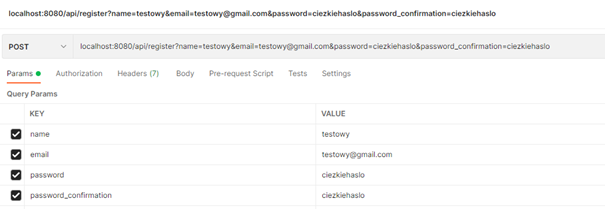
\includegraphics{zdjęcia i skriny/API_rejestracja}
\caption{Test-API Rejestracja}
\end{figure}

\begin{figure}[H]
\centering
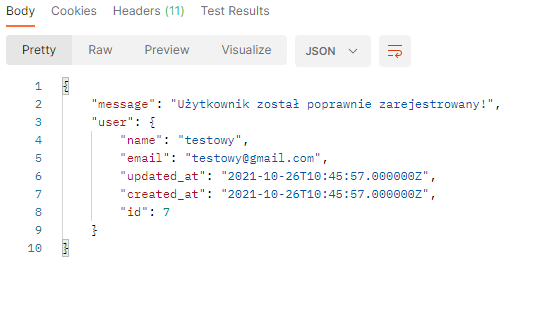
\includegraphics{zdjęcia i skriny/API_rejestracja2}
\caption{Test-API Rejestracja wynik}
\end{figure}

\item [\textbf{*}] Rejestracja z istniejącym już w bazie adresem email\\
\\
Kolejnym testem była próba, zarejestrowania użytkownika, z istniejącym już kontem w bazie danych. Test pomyślny, został zwrócony odpowiedni komunikat, informujący, że adres e-mail już istnieje w bazie.
\begin{figure}[H]
\centering
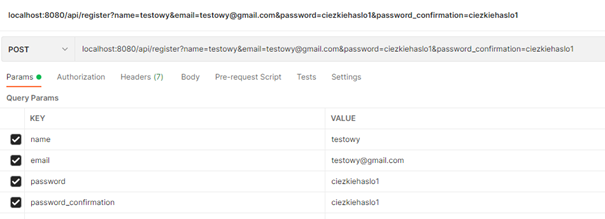
\includegraphics[width=14cm]{zdjęcia i skriny/API_rejestracjaError}
\caption{Test-API Rejestracja z istniejącym już w bazie adresem email }
\end{figure}

\begin{figure}[H]
\centering
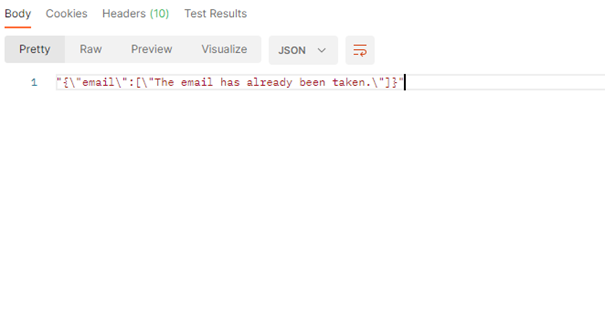
\includegraphics[width=14cm]{zdjęcia i skriny/API_rejestracjaError2}
\caption{Test-API Rejestracja z istniejącym już w bazie adresem email wynik}
\end{figure}

\item [\textbf{*}] Rejestracja bez potwierdzenia hasła\\
\\
Kolejnym testem, jest próba stworzenia konta, bez podania potwierdzenia hasła. Test dał wynik pozytywny, czego efektem jest odpowiedź, o niepasujących do siebie hasłach.
\begin{figure}[H]
\centering
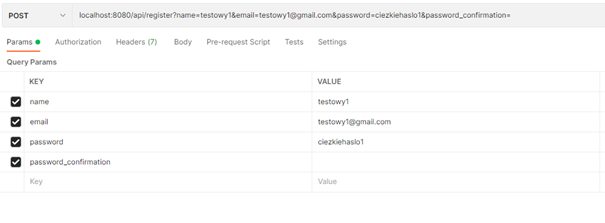
\includegraphics[width=14cm]{zdjęcia i skriny/API_rejestracjaErrorPassword}
\caption{Test-API Rejestracja bez potwierdzenia hasła}

\end{figure}
\begin{figure}[H]
\centering
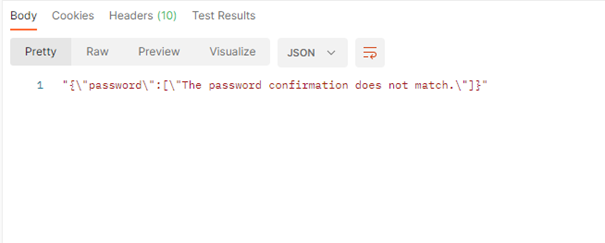
\includegraphics[width=14cm]{zdjęcia i skriny/API_rejestracjaErrorPassword2}
\caption{Test-API Rejestracja bez potwierdzenia hasła wynik}
\end{figure}

\item [\textbf{*}] Rejestracja z nieidentycznymi hasłami\\
\\
Kolejny test wykazał, że nie jest możliwa pomyślna rejestracja bez podania pasujących do siebie haseł tj. identycznych. Zwrócony został komunikat o błędzie. 
\begin{figure}[H]
\centering
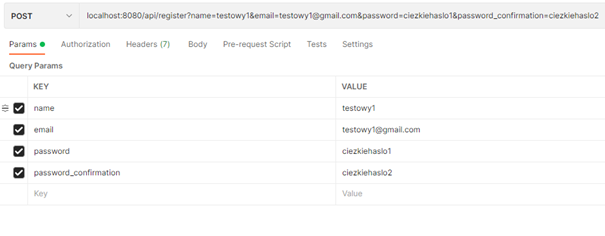
\includegraphics[width=14cm]{zdjęcia i skriny/API_rejestracjaErrorPasswordConfirm}
\caption{Test-API Rejestracja z nieidentycznymi hasłami}

\end{figure}
\begin{figure}[H]
\centering
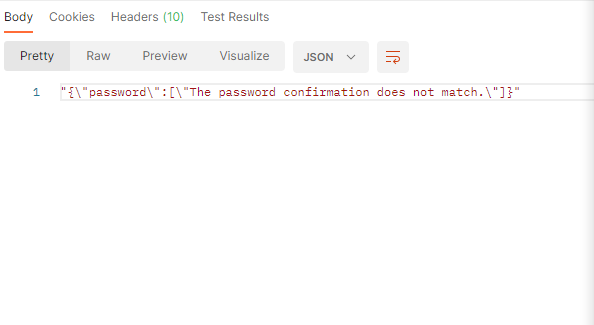
\includegraphics[width=14cm]{zdjęcia i skriny/API_rejestracjaErrorPasswordConfirm2}
\caption{Test-API Rejestracja z nieidentycznymi hasłami wynik}
\end{figure}

\item [\textbf{*}] Logowanie\\
\\
Kolejny test dotyczy logowania, po podaniu poprawnych danych logowania, wygenerowany zostaje token oraz użytkownik pomyślnie zostaje zalogowany czego efekt widzimy na poniższych screenach.
\begin{figure}[H]
\centering
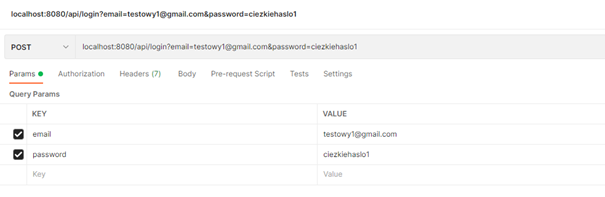
\includegraphics[width=14cm]{zdjęcia i skriny/API_login}
\caption{Test-API Logowanie}

\end{figure}
\begin{figure}[H]
\centering
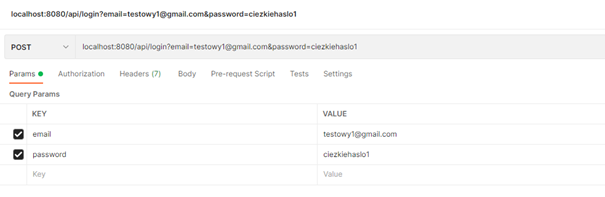
\includegraphics[width=14cm]{zdjęcia i skriny/API_login}
\caption{Test-API Logowanie}
\end{figure}

\item [\textbf{*}] Logowanie z niepoprawnym hasłem\\
\\
Kolejny test logowania, polegający na próbie zalogowania przy użyciu błędnego hasła został także pozytywnie zakończony – odpowiedni komunikat o błędzie został wyświetlony.
\begin{figure}[H]
\centering
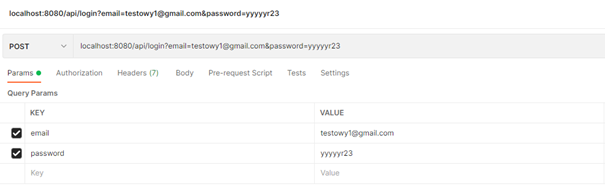
\includegraphics[width=14cm]{zdjęcia i skriny/API_loginError}
\caption{Test-API Logowanie z niepoprawnym hasłem}

\end{figure}
\begin{figure}[H]
\centering
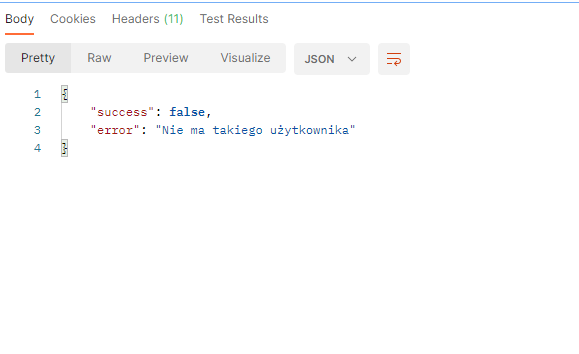
\includegraphics[width=14cm]{zdjęcia i skriny/API_loginError2}
\caption{Test-API Logowanie z niepoprawnym hasłem}
\end{figure}

\item [\textbf{*}] Logowanie bez wprowadzenia hasła\\
\\
Próba logowania z pustym polem hasła – test z wynikiem pozytywnym, wyświetlony zostaje komunikat , że pole z hasłem jest wymagane do tej czynności.
\begin{figure}[H]
\centering
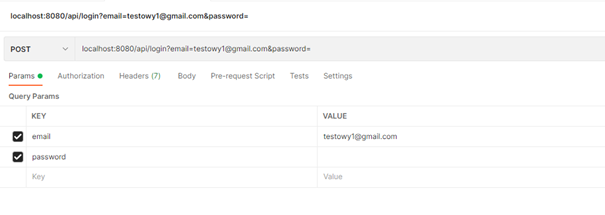
\includegraphics[width=14cm]{zdjęcia i skriny/API_loginErrorPassword}
\caption{Test-API Logowanie bez wprowadzonego hasła}

\end{figure}
\begin{figure}[H]
\centering
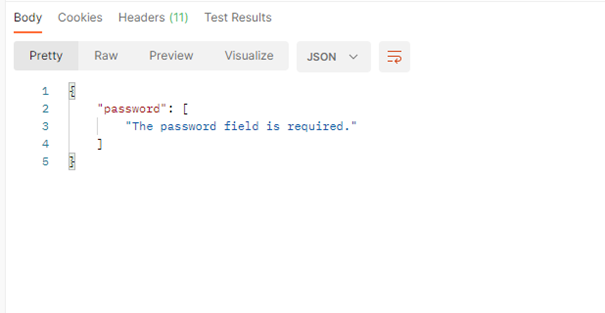
\includegraphics[width=14cm]{zdjęcia i skriny/API_loginErrorPassword2}
\caption{Test-API Logowanie  bez wprowadzonego hasła wynik}
\end{figure}

\item [\textbf{*}] Wylogowanie\\
\\
Ostatnim testem jest testowanie operacji wylogowania. Po podaniu tokenu i wysłaniu żądania, otrzymaliśmy odpowiedni komunikat o pomyślnym wylogowaniu użytkownika.
\begin{figure}[H]
\centering
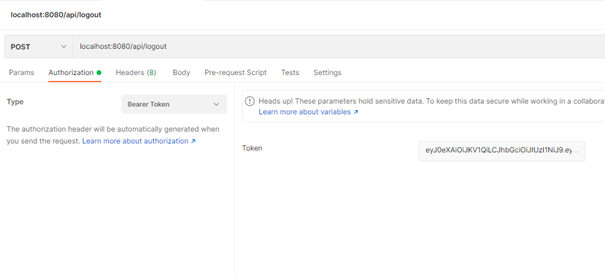
\includegraphics[width=14cm]{zdjęcia i skriny/API_logout}
\caption{Test-API Wylogowanie}
\end{figure}


\begin{figure}[H]
\centering
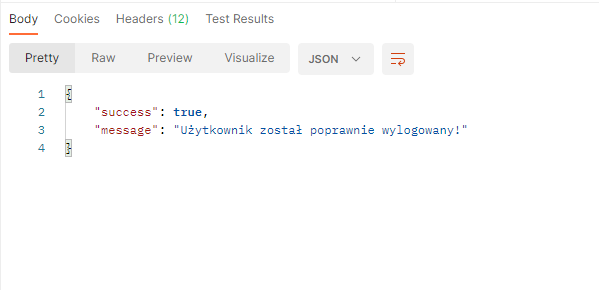
\includegraphics[width=14cm]{zdjęcia i skriny/API_logout2}
\caption{Test-API Wylogowanie wynik}
\end{figure}
\end{itemize}


\section{Podsumowanie i bilans}
(MVP vs rzeczywistość)





\newpage


\section{Layout aplikacji SINGIEL 2.0}
\begin{figure}[H]
\centering
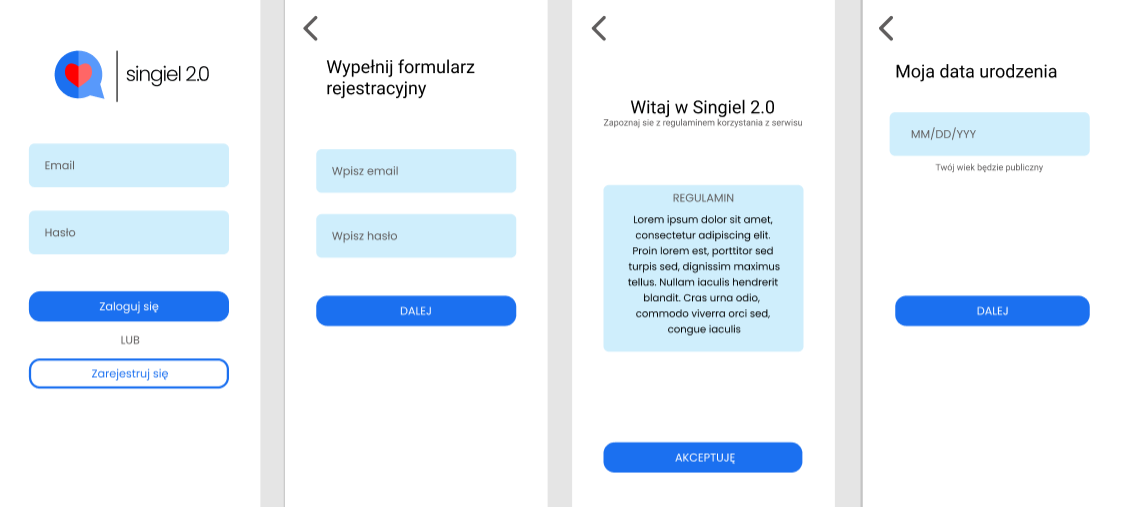
\includegraphics[width=14cm]{zdjęcia i skriny/log1.PNG}
\caption{Rejestracja i logowanie}
\end{figure}

\begin{figure}[H]
\centering
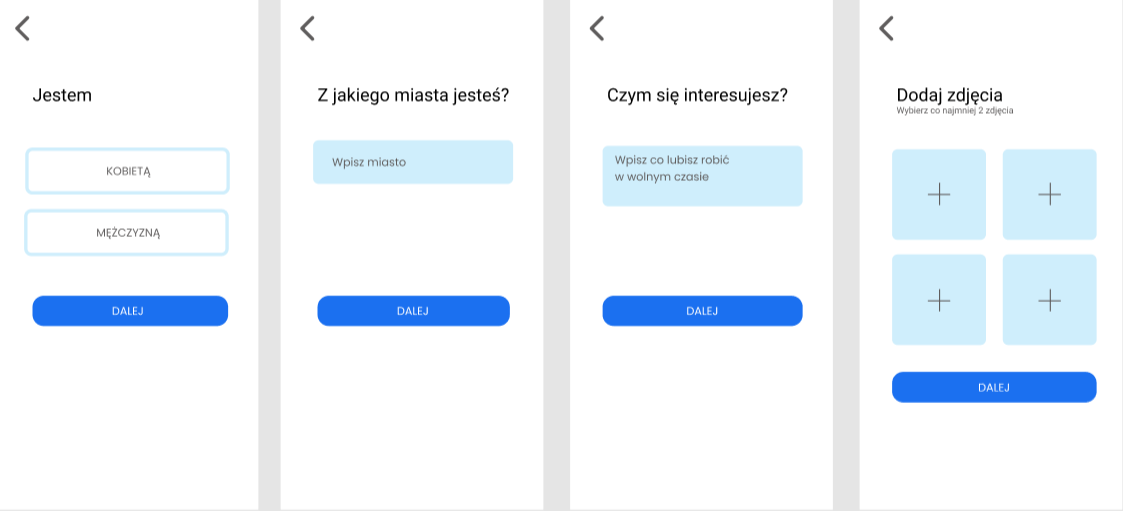
\includegraphics[width=14cm]{zdjęcia i skriny/log2.PNG}
\caption{Rejestracja i logowanie}
\end{figure}


\begin{figure}[H]
\centering
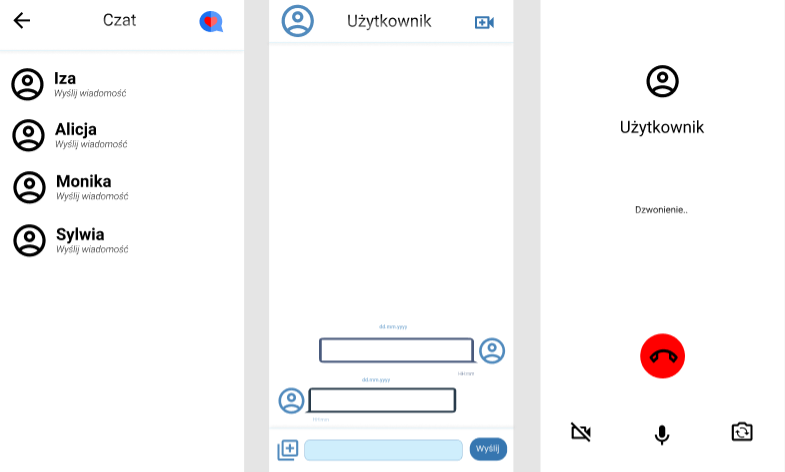
\includegraphics[width=15cm]{zdjęcia i skriny/czat1.PNG}
\caption{Czatowanie i wideo rozmowa}
\end{figure}

\begin{figure}[H]
\centering
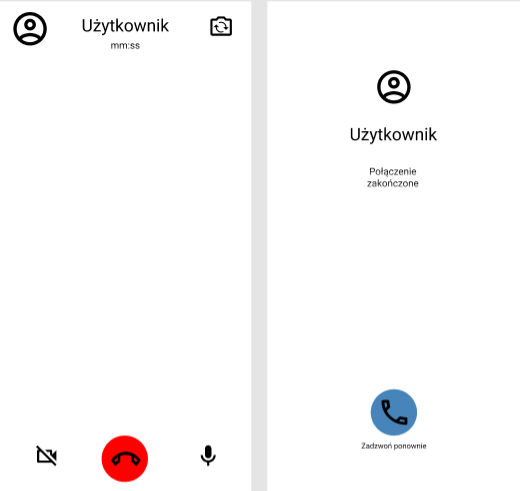
\includegraphics[width=10cm]{zdjęcia i skriny/czat2.PNG}
\caption{Czatowanie i wideo rozmowa}
\end{figure}

\begin{figure}[H]
\centering
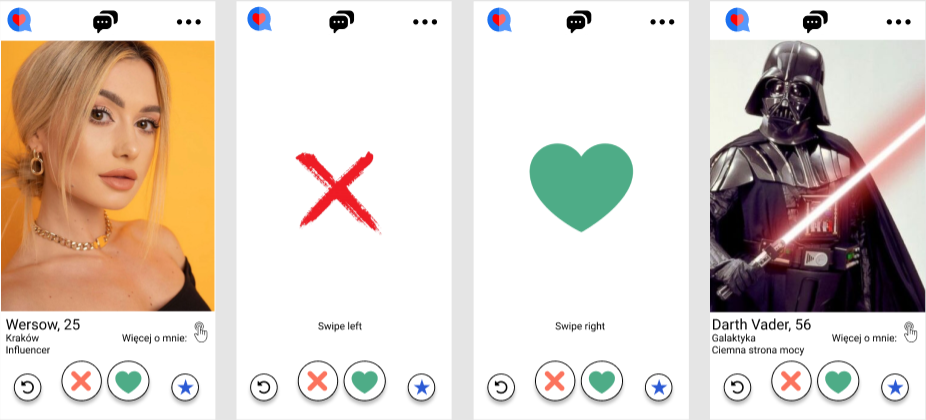
\includegraphics[width=15cm]{zdjęcia i skriny/swipe up.PNG}
\caption{Swipe up}
\end{figure}

\begin{figure}[H]
\centering
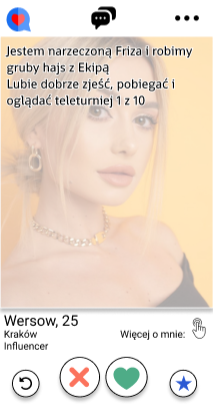
\includegraphics[width=5cm]{zdjęcia i skriny/swipe 2.PNG}
\caption{Opis użytkownika}
\end{figure}


\begin{figure}[H]
\centering
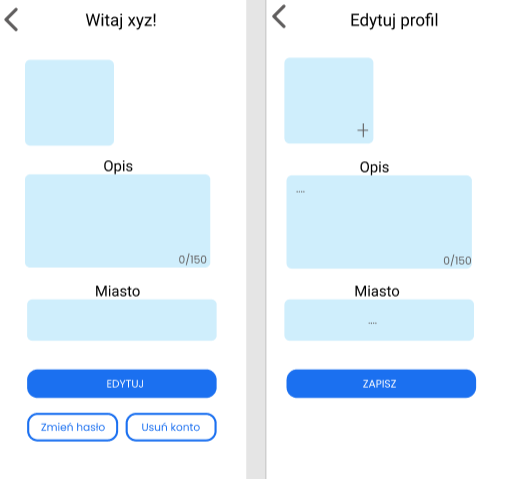
\includegraphics[width=9cm]{zdjęcia i skriny/edycja.PNG}
\caption{Edycja profilu}
\end{figure}

\newpage
\begin{thebibliography}{9}
\bibitem{java1} {\it Opis języków programowania - Java} (\url{https://en.wikipedia.org/wiki/Android_software_development}).
\bibitem{java2} {\it Języki programowania w androidzie} (\url{https://www.androidauthority.com/develop-android-apps-languages-learn-391008/}).
\bibitem{firebase} {\it Firebase opis technologii} (\url{https://bugajsky.pl/2019/07/31/czym-jest-firebase/}).
\bibitem{webrtc} {\it WebRtc dokumentacja} (\url{https://webrtc.org/}).
\bibitem{webrtcWikipedia} {\it WebRtc Wikipedia} (\url{https://pl.wikipedia.org/wiki/WebRTC}).
\bibitem{xml} {\it Technologia XML} (\url{https://pl.wikipedia.org/wiki/XML}).
\end{thebibliography}

\end{document}

